\documentclass{standalone}
\usepackage{tikz}
\usetikzlibrary{patterns, positioning}
\usepackage[sfdefault]{ClearSans} %% option 'sfdefault' activates Clear Sans as the default text font
\usepackage[T1]{fontenc}

\begin{document}
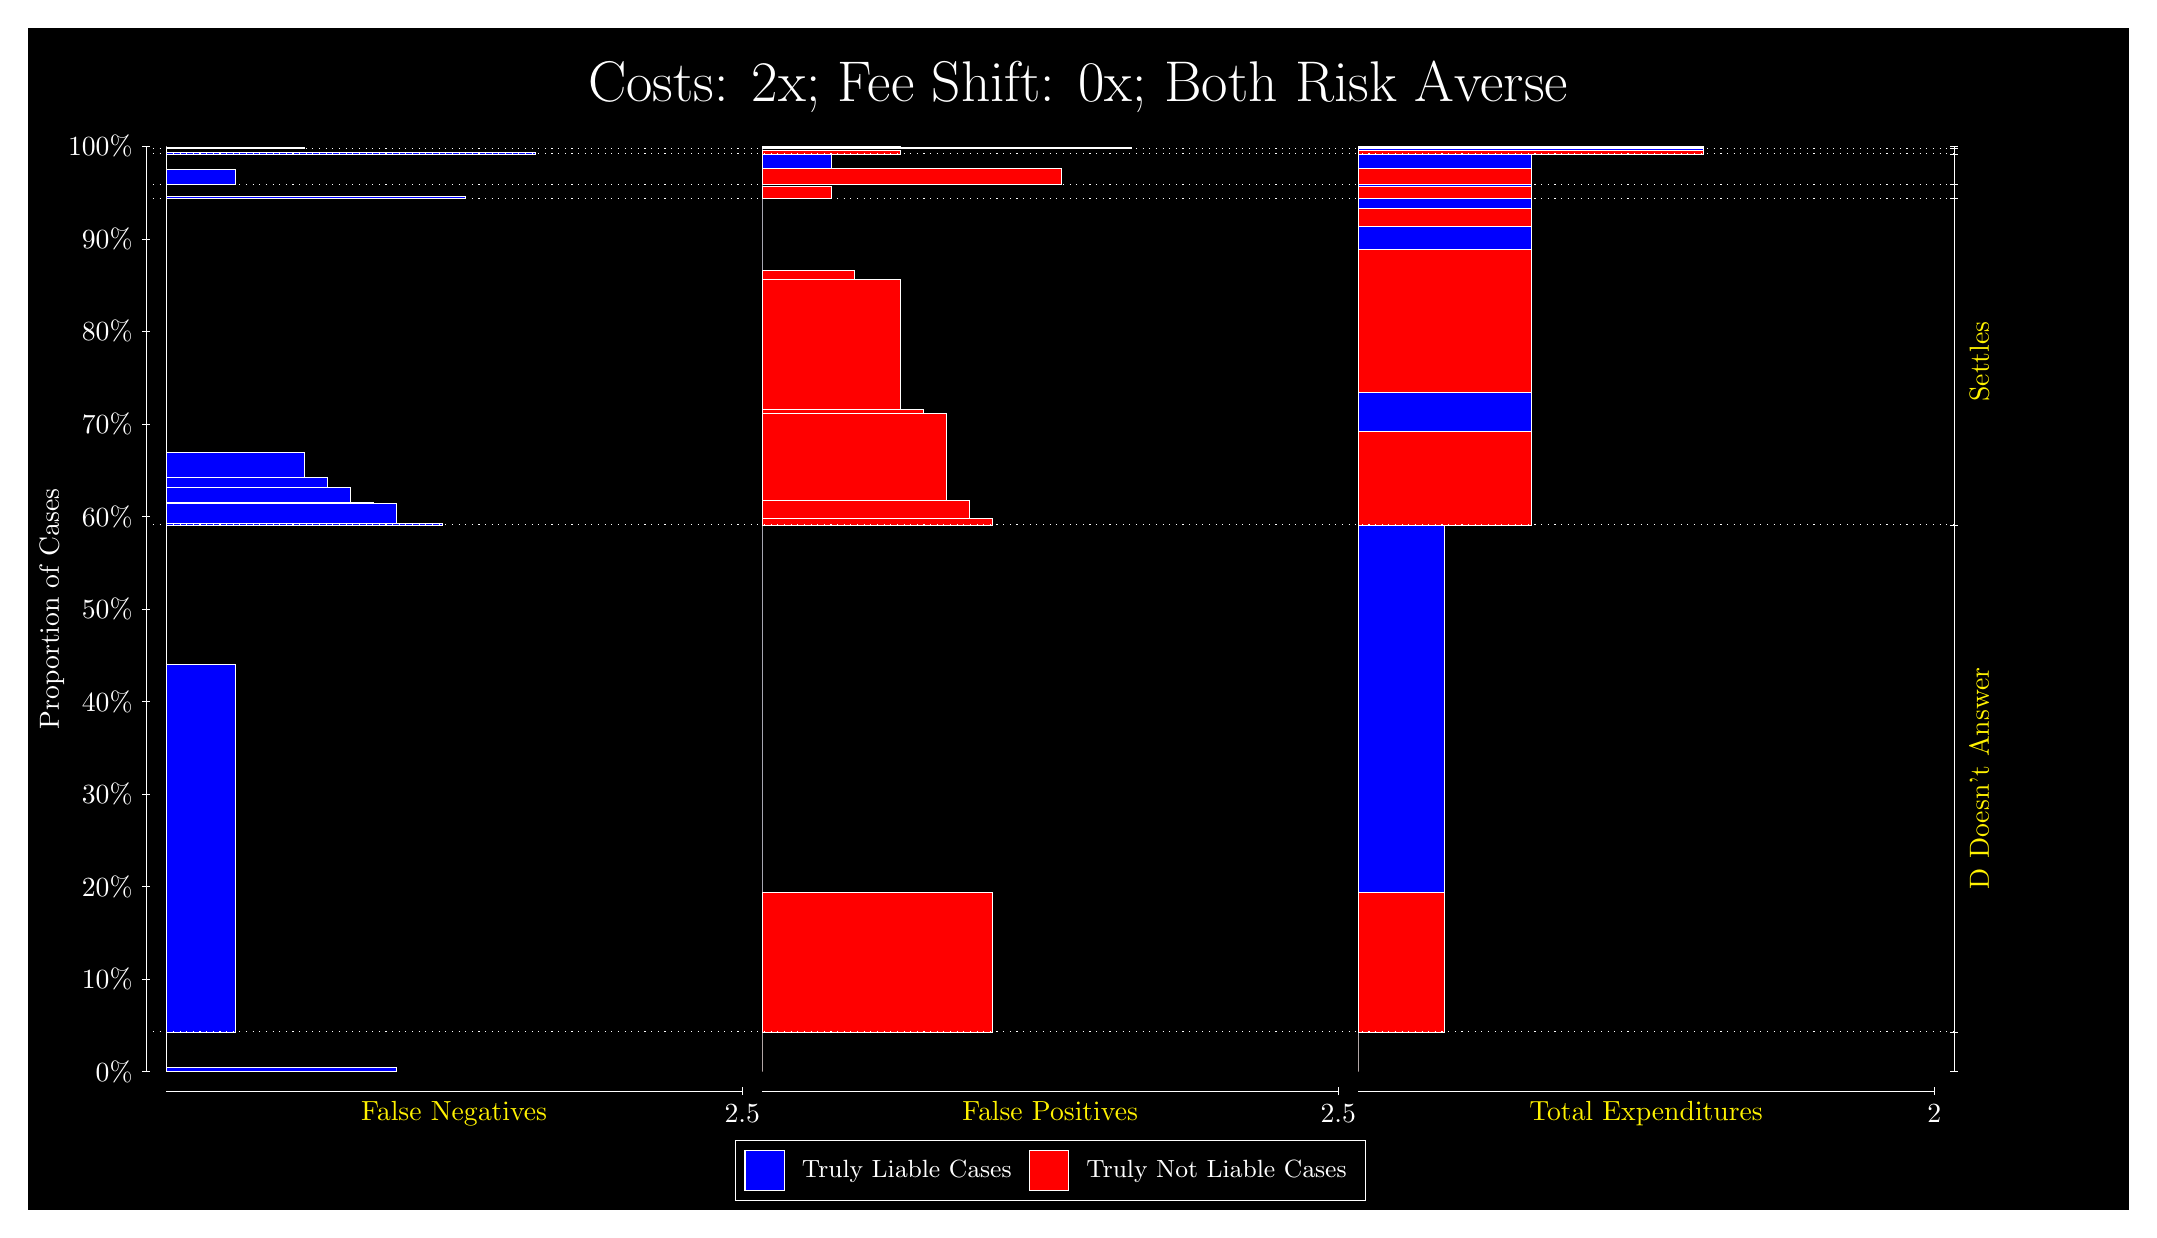
\begin{tikzpicture}
\draw[fill=black] (0,0) rectangle (26.667,15);
\draw[text=white] (0,13.5) rectangle (26.667,15) node[midway] {\huge Costs: 2x; Fee Shift: 0x; Both Risk Averse};
\draw[white, very thin] (1.5,1.75) -- (1.5,13.5);
\node[rotate=90, text=white, anchor=center] at (0.3, 7.625) {Proportion of Cases};
\draw[white, very thin] (1.45,1.75) -- (1.55,1.75);
\node[text=white, anchor=east] at (1.45, 1.75) {0\%};
\draw[white, very thin] (1.45,2.925) -- (1.55,2.925);
\node[text=white, anchor=east] at (1.45, 2.925) {10\%};
\draw[white, very thin] (1.45,4.1) -- (1.55,4.1);
\node[text=white, anchor=east] at (1.45, 4.1) {20\%};
\draw[white, very thin] (1.45,5.275) -- (1.55,5.275);
\node[text=white, anchor=east] at (1.45, 5.275) {30\%};
\draw[white, very thin] (1.45,6.45) -- (1.55,6.45);
\node[text=white, anchor=east] at (1.45, 6.45) {40\%};
\draw[white, very thin] (1.45,7.625) -- (1.55,7.625);
\node[text=white, anchor=east] at (1.45, 7.625) {50\%};
\draw[white, very thin] (1.45,8.8) -- (1.55,8.8);
\node[text=white, anchor=east] at (1.45, 8.8) {60\%};
\draw[white, very thin] (1.45,9.975) -- (1.55,9.975);
\node[text=white, anchor=east] at (1.45, 9.975) {70\%};
\draw[white, very thin] (1.45,11.15) -- (1.55,11.15);
\node[text=white, anchor=east] at (1.45, 11.15) {80\%};
\draw[white, very thin] (1.45,12.325) -- (1.55,12.325);
\node[text=white, anchor=east] at (1.45, 12.325) {90\%};
\draw[white, very thin] (1.45,13.5) -- (1.55,13.5);
\node[text=white, anchor=east] at (1.45, 13.5) {100\%};

\draw[white, very thin] (24.457,1.75) -- (24.457,13.5);
\draw[white, very thin] (24.407,1.75) -- (24.507,1.75);
\node[anchor=west] at (24.407, 1.75) {};
\draw[white, very thin] (24.407,2.2545) -- (24.507,2.2545);
\node[anchor=west] at (24.407, 2.2545) {};
\draw[white, very thin] (24.407,8.6936) -- (24.507,8.6936);
\node[anchor=west] at (24.407, 8.6936) {};
\draw[white, very thin] (24.407,12.841) -- (24.507,12.841);
\node[anchor=west] at (24.407, 12.841) {};
\draw[white, very thin] (24.407,13.016) -- (24.507,13.016);
\node[anchor=west] at (24.407, 13.016) {};
\draw[white, very thin] (24.407,13.405) -- (24.507,13.405);
\node[anchor=west] at (24.407, 13.405) {};
\draw[white, very thin] (24.407,13.471) -- (24.507,13.471);
\node[anchor=west] at (24.407, 13.471) {};
\draw[white, very thin] (24.407,13.5) -- (24.507,13.5);
\node[anchor=west] at (24.407, 13.5) {};

\draw[white, very thin, fill=blue] (1.75,1.75) rectangle (4.6775,1.8031);
\draw[white, very thin, fill=red] (1.75,1.8031) rectangle (1.75,2.2545);
\draw[white, very thin, fill=blue] (1.75,2.2545) rectangle (2.6283,6.9166);
\draw[white, very thin, fill=red] (1.75,6.9166) rectangle (1.75,8.6936);
\draw[white, very thin, fill=blue] (1.75,8.6936) rectangle (5.2631,8.7113);
\draw[white, very thin, fill=blue] (1.75,8.7113) rectangle (4.6775,8.9702);
\draw[white, very thin, fill=blue] (1.75,8.9702) rectangle (4.3848,8.9822);
\draw[white, very thin, fill=blue] (1.75,8.9822) rectangle (4.092,9.1672);
\draw[white, very thin, fill=blue] (1.75,9.1672) rectangle (3.7993,9.294);
\draw[white, very thin, fill=blue] (1.75,9.294) rectangle (3.5065,9.6082);
\draw[white, very thin, fill=red] (1.75,9.6082) rectangle (1.75,12.841);
\draw[white, very thin, fill=blue] (1.75,12.841) rectangle (5.5558,12.866);
\draw[white, very thin, fill=red] (1.75,12.866) rectangle (1.75,13.016);
\draw[white, very thin, fill=blue] (1.75,13.016) rectangle (2.6283,13.207);
\draw[white, very thin, fill=red] (1.75,13.207) rectangle (1.75,13.405);
\draw[white, very thin, fill=blue] (1.75,13.405) rectangle (6.4341,13.42);
\draw[white, very thin, fill=red] (1.75,13.42) rectangle (1.75,13.471);
\draw[white, very thin, fill=blue] (1.75,13.471) rectangle (3.5065,13.485);
\draw[white, very thin, fill=red] (1.75,13.485) rectangle (1.75,13.5);
\draw[white, very thin, fill=red] (9.3189,1.75) rectangle (9.3189,2.2015);
\draw[white, very thin, fill=blue] (9.3189,2.2015) rectangle (9.3189,2.2545);
\draw[white, very thin, fill=red] (9.3189,2.2545) rectangle (12.246,4.0315);
\draw[white, very thin, fill=blue] (9.3189,4.0315) rectangle (9.3189,8.6936);
\draw[white, very thin, fill=red] (9.3189,8.6936) rectangle (12.246,8.7704);
\draw[white, very thin, fill=red] (9.3189,8.7704) rectangle (11.954,9.0053);
\draw[white, very thin, fill=red] (9.3189,9.0053) rectangle (11.661,10.111);
\draw[white, very thin, fill=red] (9.3189,10.111) rectangle (11.368,10.155);
\draw[white, very thin, fill=red] (9.3189,10.155) rectangle (11.075,11.815);
\draw[white, very thin, fill=red] (9.3189,11.815) rectangle (10.49,11.926);
\draw[white, very thin, fill=blue] (9.3189,11.926) rectangle (9.3189,12.841);
\draw[white, very thin, fill=red] (9.3189,12.841) rectangle (10.197,12.991);
\draw[white, very thin, fill=blue] (9.3189,12.991) rectangle (9.3189,13.016);
\draw[white, very thin, fill=red] (9.3189,13.016) rectangle (13.125,13.215);
\draw[white, very thin, fill=blue] (9.3189,13.215) rectangle (10.197,13.405);
\draw[white, very thin, fill=red] (9.3189,13.405) rectangle (11.075,13.456);
\draw[white, very thin, fill=blue] (9.3189,13.456) rectangle (9.3189,13.471);
\draw[white, very thin, fill=red] (9.3189,13.471) rectangle (14.003,13.485);
\draw[white, very thin, fill=blue] (9.3189,13.485) rectangle (11.075,13.5);
\draw[white, very thin, fill=red] (16.888,1.75) rectangle (16.888,2.2015);
\draw[white, very thin, fill=blue] (16.888,2.2015) rectangle (16.888,2.2545);
\draw[white, very thin, fill=red] (16.888,2.2545) rectangle (17.986,4.0315);
\draw[white, very thin, fill=blue] (16.888,4.0315) rectangle (17.986,8.6936);
\draw[white, very thin, fill=red] (16.888,8.6936) rectangle (19.083,9.8757);
\draw[white, very thin, fill=blue] (16.888,9.8757) rectangle (19.083,10.375);
\draw[white, very thin, fill=red] (16.888,10.375) rectangle (19.083,12.19);
\draw[white, very thin, fill=blue] (16.888,12.19) rectangle (19.083,12.479);
\draw[white, very thin, fill=red] (16.888,12.479) rectangle (19.083,12.714);
\draw[white, very thin, fill=blue] (16.888,12.714) rectangle (19.083,12.841);
\draw[white, very thin, fill=red] (16.888,12.841) rectangle (19.083,12.991);
\draw[white, very thin, fill=blue] (16.888,12.991) rectangle (19.083,13.016);
\draw[white, very thin, fill=red] (16.888,13.016) rectangle (19.083,13.215);
\draw[white, very thin, fill=blue] (16.888,13.215) rectangle (19.083,13.405);
\draw[white, very thin, fill=red] (16.888,13.405) rectangle (21.279,13.456);
\draw[white, very thin, fill=blue] (16.888,13.456) rectangle (21.279,13.471);
\draw[white, very thin, fill=red] (16.888,13.471) rectangle (21.279,13.485);
\draw[white, very thin, fill=blue] (16.888,13.485) rectangle (21.279,13.5);
\draw[white, dotted] (1.5,2.2545) -- (24.457,2.2545);
\draw[white, dotted] (1.5,8.6936) -- (24.457,8.6936);
\draw[white, dotted] (1.5,12.841) -- (24.457,12.841);
\draw[white, dotted] (1.5,13.016) -- (24.457,13.016);
\draw[white, dotted] (1.5,13.405) -- (24.457,13.405);
\draw[white, dotted] (1.5,13.471) -- (24.457,13.471);
\draw[white, very thin] (1.75,1.5) -- (9.0689,1.5);
\node[text=yellow, anchor=north] at (5.4094, 1.5) {False Negatives};
\draw[white, very thin] (9.0689,1.45) -- (9.0689,1.55);
\node[text=white, anchor=north] at (9.0689, 1.45) {2.5};

\draw[white, very thin] (9.3189,1.5) -- (16.638,1.5);
\node[text=yellow, anchor=north] at (12.978, 1.5) {False Positives};
\draw[white, very thin] (16.638,1.45) -- (16.638,1.55);
\node[text=white, anchor=north] at (16.638, 1.45) {2.5};

\draw[white, very thin] (16.888,1.5) -- (24.207,1.5);
\node[text=yellow, anchor=north] at (20.547, 1.5) {Total Expenditures};
\draw[white, very thin] (24.207,1.45) -- (24.207,1.55);
\node[text=white, anchor=north] at (24.207, 1.45) {2};


\node[text=yellow, centered, rotate=90] at (24.777, 5.474) {D Doesn't Answer};
\node[text=yellow, centered, rotate=90] at (24.777, 10.767) {Settles};





\draw (12.978300999999998,1.5) node[draw=none] (baseCoordinate) {};
\begin{scope}[align=center]
        \matrix[scale=0.5, draw=white, below=0.5cm of baseCoordinate, nodes={draw}, column sep=0.1cm]{
            \node[rectangle, draw, minimum width=0.5cm, minimum height=0.5cm, fill=blue] {}; &
            \node[draw=none, font=\small, text=white] (B) {Truly Liable Cases}; &
            \node[rectangle, draw, minimum width=0.5cm, minimum height=0.5cm, fill=red] {}; &
            \node[draw=none, font=\small, text=white] (B) {Truly Not Liable Cases}; \\
            };
\end{scope}

\end{tikzpicture}
\end{document}